
\begin{figure}[h]
    \centering
    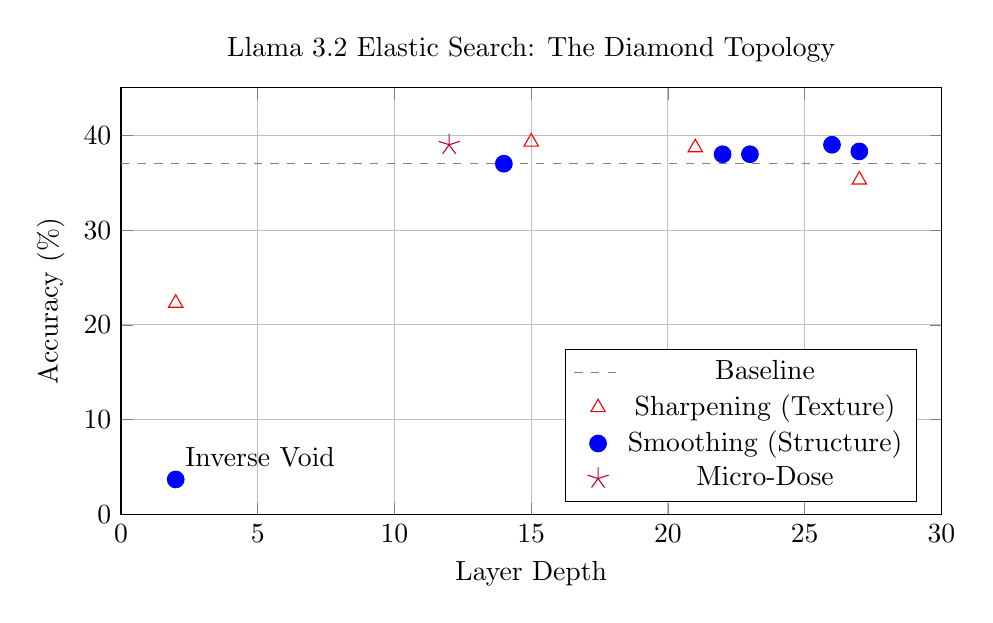
\begin{tikzpicture}
        \begin{axis}[
            title={Llama 3.2 Elastic Search: The Diamond Topology},
            xlabel={Layer Depth},
            ylabel={Accuracy (\%)},
            xmin=0, xmax=30,
            ymin=0, ymax=45,
            grid=major,
            legend pos=south east,
            width=12cm, height=7cm
        ]
        
        % Baseline
        \addplot[dashed, gray, domain=0:30] {37.0};
        \addlegendentry{Baseline}
        
        % Sharpening
        \addplot[mark=triangle, red, mark size=3pt, only marks] coordinates {
            (2, 22.3) (15, 39.3) (21, 38.7) (27, 35.3)
        };
        \addlegendentry{Sharpening (Texture)}
        
        % Smoothing
        \addplot[mark=*, blue, mark size=3pt, only marks] coordinates {
            (2, 3.7) (14, 37.0) (22, 38.0) (23, 38.0) (26, 39.0) (27, 38.3)
        };
        \addlegendentry{Smoothing (Structure)}
        
        % Micro-Dose
        \addplot[mark=star, purple, mark size=4pt, only marks] coordinates {
            (12, 39.0)
        };
        \addlegendentry{Micro-Dose}
        
        % Annotation
        \node[anchor=south west] at (axis cs: 2, 4) {Inverse Void};
        
        \end{axis}
    \end{tikzpicture}
    \caption{Exhaustive sweep of Llama 3.2 layers. It rejects most interventions ("Diamond"), with a specific Inverse Void at Layer 2 and minor Texture/Safety peaks.}
    \label{fig:llama_elastic}
\end{figure}
